\documentclass[10pt]{beamer}

\usepackage[english]{babel}
\usepackage[utf8]{inputenc}
\usepackage{amsmath,amssymb,amsthm,latexsym}
\usepackage{mathrsfs}
\usepackage[all]{xypic}
\usepackage{tikz}
\usetikzlibrary{arrows,shapes,automata}
\usepackage{eurosym}
\usepackage{listings}
\usepackage{textcomp}

\newcommand{\cat}[1]{\mathscr{#1}}
\newcommand{\lcat}[1]{\mathbf{#1}}
\newcommand{\C}{\cat{C}}
\newcommand{\D}{\cat{D}}
\renewcommand{\L}{\cat{L}}
\newcommand{\comp}{\circ}
\newcommand{\size}[1]{\lVert#1\rVert}
\newcommand{\sizein}[1]{\size{#1}^\mathrm{in}}
\newcommand{\sizeout}[1]{\size{#1}_\mathrm{out}}
\DeclareMathOperator{\ob}{ob}
\DeclareMathOperator{\Hom}{Hom}
\DeclareMathOperator{\id}{id}
\DeclareMathOperator{\Id}{Id}
\newcommand{\N}{\mathbb{N}}
\newcommand{\Z}{\mathbb{Z}}
\newcommand{\Complex}{\mathbb{C}}
\newcommand{\R}{\mathbb{R}}
\newcommand{\K}{\mathbb{K}}
\newcommand{\LK}{\mathbb{L}}
\newcommand{\ra}{\rightarrow}
\newcommand{\la}{\leftarrow}
\DeclareMathOperator{\Time}{t}
\DeclareMathOperator{\Space}{s}
\DeclareMathOperator{\coTime}{co-t}
\DeclareMathOperator{\coSpace}{co-s}
\DeclareMathOperator{\Par}{Par}
\DeclareMathOperator{\Tr}{Tr}
\DeclareMathOperator{\rev}{rev}
\newcommand{\computes}{\vdash}
\renewcommand{\u}{\underline}
\renewcommand{\o}{\overline}
\newcommand{\tALpy}{\texttt{transalpyne}}


\mode<presentation>{%
  \usetheme[]{Madrid}
  \usecolortheme{seahorse}
  \usecolortheme{rose}
  \usefonttheme[onlymath]{serif}
}


\title{On the transposition of computer programs}
\author[L. De Feo]{L.~De~Feo\\{\footnotesize(joint work with É.~Schost)}}
\institute[TANC, LIX]{Projet TANC, LIX, École Polytechnique}
\date[Bonn, June 10, 2010]{COSEC Seminar, \textbf{b}-it\\ Bonn, June 10, 2010}

\AtBeginSection[]
{
  \begin{frame}<beamer>
    \frametitle{Plan}
    \tableofcontents[currentsection]
  \end{frame}
}


\begin{document}

\begin{frame}
  \titlepage
\end{frame}

%%
%%

\section{The transposition principle}

\begin{frame}
  \frametitle{Arithmetic circuits}

  \begin{block}{Algebraic complexity}
    \centering Fix a ring $R$. We construct circuits that evaluate
    arithmetic functions.
  \end{block}


  \begin{center}
    Three gates: Addition, duplication, multiplication by a fixed
    element $a\in R$.
    
    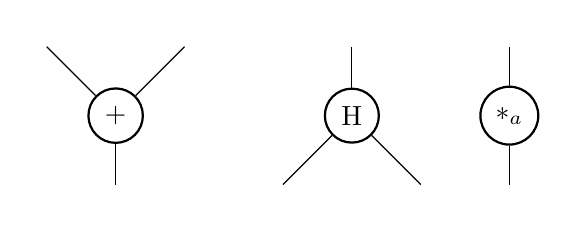
\begin{tikzpicture}
      \tikzstyle{node}=[circle,thick,draw=black,minimum size=4mm]
      
      \begin{scope}
        \node(in1){};
        \node(nop1)[right of=in1]{};
        \node(in2)[right of=nop1]{};
        \node(nop2)[right of=in2]{};
        \node(in3)[right of=nop2]{};
        \node(nop3)[right of=in3]{};
        \node(in4)[right of=nop3]{};
        
        \node[node](plus)[below of=nop1]{$+$}
        edge(in1)
        edge(in2);
        \node(nop)[below of=nop2]{};
        \node[node](hub)[below of=in3]{H}
        edge(in3);
        \node[node](times)[below of=in4]{$*_a$}
        edge(in4);
        
        \node(out1)[below of=plus]{}
        edge(plus);
        \node(nop5)[right of=out1]{};
        \node(out2)[below of=nop]{}
        edge(hub);
        \node(nop6)[below of=hub]{};
        \node(out3)[right of=nop6]{}
        edge(hub);
        \node(out4)[below of=times]{}
        edge(times);
      \end{scope}
    \end{tikzpicture}
  \end{center}
\end{frame}

%%

\begin{frame}
  \frametitle{Arithmetic circuits}

  \begin{columns}
    \begin{column}{0.6\textwidth}
      \centering
      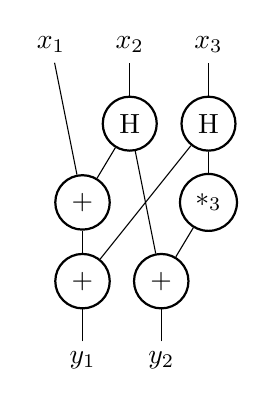
\begin{tikzpicture}
        \tikzstyle{node}=[circle,thick,draw=black,minimum size=4mm]
        
        \begin{scope}
          \node(x1){$x_1$};
          \node(x2)[right of=x1]{$x_2$};
          \node(x3)[right of=x2]{$x_3$};
          
          \node[node](d1)[below of=x2]{H}
          edge(x2);
          \node[node](d2)[below of=x3]{H}
          edge(x3);
          
          \node[node](p1)[below of=d1,xshift=-6mm]{$+$}
          edge(x1)
          edge(d1);
          \node[node](m1)[below of=d2]{$*_3$}
          edge(d2);
          
          \node[node](p2)[below of=p1]{$+$}
          edge(p1)
          edge(d2);
          \node[node](p3)[right of=p2]{$+$}
          edge(d1)
          edge(m1);
          
          \node(y1)[below of=p2]{$y_1$}
          edge(p2);
          \node(y2)[below of=p3]{$y_2$}
          edge(p3);
        \end{scope}
      \end{tikzpicture}
    \end{column}
    \begin{column}{0.4\textwidth}
      \begin{align*}
        y_1 &= x_1 + x_2 + x_3\\
        y_2 &= x_2 + 3x_3
      \end{align*}
      
      \Large
      \begin{gather*}
        \begin{pmatrix}
          1 & 1 & 1\\
          0 & 1 & 3
        \end{pmatrix}
      \end{gather*}
    \end{column}
  \end{columns}
\end{frame}

%%

\begin{frame}
  \frametitle{Transposition of an arithmetic circuit}

  \begin{columns}
    \begin{column}{0.6\textwidth}
      \centering
      \begin{tikzpicture}
        \tikzstyle{node}=[circle,thick,draw=black,minimum size=4mm]
        
        \begin{scope}
          \node(x1){$x_1$};
          \node(x2)[right of=x1]{$x_2$};
          \node(x3)[right of=x2]{$x_3$};
          
          \node[node](d1)[below of=x2]{H}
          edge(x2);
          \node[node](d2)[below of=x3]{H}
          edge(x3);
            
          \node[node](p1)[below of=d1,xshift=-6mm]{$+$}
          edge(x1)
          edge(d1);
          \node[node](m1)[below of=d2]{$*_3$}
          edge(d2);
          
          \node[node](p2)[below of=p1]{$+$}
          edge(p1)
          edge(d2);
          \node[node](p3)[right of=p2]{$+$}
          edge(d1)
          edge(m1);
          
          \node(y1)[below of=p2]{$y_1$}
          edge(p2);
          \node(y2)[below of=p3]{$y_2$}
          edge(p3);
        \end{scope}
        
        \begin{scope}[xshift=3.2cm, yshift=-0.23\textheight]
          \node(x){\Huge $\leftrightarrow$};
        \end{scope}
        
        \begin{scope}[xshift=4cm, yshift=-0.425\textheight]
          \node(x1){$x_1'$};
          \node(x2)[right of=x1]{$x_2'$};
          \node(x3)[right of=x2]{$x_3'$};
          
          \node[node](d1)[above of=x2]{\alt<2>{$+$}{H}}
          edge(x2);
          \node[node](d2)[above of=x3]{\alt<2>{$+$}{H}}
          edge(x3);
          
          \node[node](p1)[above of=d1,xshift=-5mm]{\alt<2>{H}{$+$}}
          edge(x1)
          edge(d1);
          \node[node](m1)[above of=d2]{$*_3$}
          edge(d2);
          
          \node[node](p2)[above of=p1]{\alt<2>{H}{$+$}}
          edge(p1)
          edge(d2);
          \node[node](p3)[right of=p2]{\alt<2>{H}{$+$}}
          edge(d1)
          edge(m1);
          
          \node(y1)[above of=p2]{$y_1'$}
          edge(p2);
          \node(y2)[above of=p3]{$y_2'$}
          edge(p3);
        \end{scope}
      \end{tikzpicture}
    \end{column}
    \begin{column}{0.4\textwidth}
      \begin{align*}
        y_1 &= x_1 + x_2 + x_3\\
        y_2 &= x_2 + 3x_3
      \end{align*}
      
      \Large
      \begin{gather*}
        \begin{pmatrix}
          1 & 1 & 1\\
          0 & 1 & 3
        \end{pmatrix}\\
        \updownarrow\\
        \begin{pmatrix}
          1 & 0\\
          1 & 1\\
          1 & 3\\
        \end{pmatrix}
      \end{gather*}
    \end{column}
  \end{columns}
\end{frame}

%%
%%

\begin{frame}
  \frametitle{Arithmetic Circuits: uniform vs. non-uniform}

  \begin{definition}[Circuit family]
    A \emph{circuit family} is a family $(C_0,C_1,\ldots)$ of circuits
    indexed by $\N$ such that $C_n$ has $n$ inputs.
  \end{definition}

  \begin{definition}[Uniform circuit family]
    A circuit family $(C_0,C_1,\ldots)$ is said to be \emph{uniform}
    if there is a $\log n$-space bounded touring machine which on
    input $1^n$ outputs a representation of $C_n$.
  \end{definition}

  \begin{itemize}
  \item We will extend the definition to allow families to be indexed
    by any (countable) set $\mathcal{P}$, called the \emph{parameter
      space}.
  \item \alert{Any Touring-undecidable problem has a trivial
      \emph{polynomial-size} non-uniform circuit family deciding it.}
  \end{itemize}
\end{frame}

%%

\begin{frame}[fragile]
  \frametitle{From non-uniform to uniform circuits?}
  
  {\large
    \begin{itemize}
    \item The transposition theorem easily generalises to non-uniform
      circuits.
    \item It can even be directly applied to computer programs (under
      certain hypotheses).
    \end{itemize}}

    \begin{columns}

    \begin{column}{0.5\textwidth}
      \begin{center}
        \begin{minipage}{0.7\textwidth}
\begin{semiverbatim}
  for i = 0 to n-2 do
    a[i+1] = a[i] + a[i+1]
    a[i] = 0
  end for
\end{semiverbatim}
        \end{minipage}
      \end{center}
    \end{column}

    \begin{column}{0.5\textwidth}

      \begin{equation*}
        \begin{pmatrix}
          0 & \hdotsfor{3} & 0\\
          \vdots  &  &\vdots&& \vdots \\
          0 & \hdotsfor{3} & 0\\
          1 & \hdotsfor{3} & 1
        \end{pmatrix}
      \end{equation*}

    \end{column}
  \end{columns}


\end{frame}

%%

\begin{frame}[fragile]
  \frametitle{From non-uniform to uniform circuits?}

  \begin{columns}
    \begin{column}{0.5\textwidth}
      \begin{center}
        \begin{minipage}{0.7\textwidth}
\begin{semiverbatim}
  a[1] = a[0] + a[1]
  a[0] = 0
  a[2] = a[1] + a[2]
  a[1] = 0
  ...
  a[n-1] = a[n-2] + a[n-1]
  a[n-2] = 0
\end{semiverbatim}
        \end{minipage}
      \end{center}
    \end{column}

    \begin{column}{0.5\textwidth}
      \begin{center}
        \begin{minipage}{0.7\textwidth}
\begin{semiverbatim}
  a[n-2] = 0
  a[n-2] = a[n-2] + a[n-1]
  ...
  a[1] = 0
  a[1] = a[1] + a[2]
  a[0] = 0
  a[0] = a[0] + a[1]
\end{semiverbatim}
        \end{minipage}
      \end{center}
    \end{column}
    \end{columns}
  
  \vfill

  \begin{columns}

    \begin{column}{0.5\textwidth}
      \begin{center}
        \begin{minipage}{0.7\textwidth}
\begin{semiverbatim}
  for i = n-2 to 0 do
    a[i] = 0
    a[i] = a[i] + a[i+1]
  end for
\end{semiverbatim}
        \end{minipage}
      \end{center}
    \end{column}

    \begin{column}{0.5\textwidth}

      \begin{equation*}
        \begin{pmatrix}
          0 & \hdotsfor{3} & 0\\
          \vdots  &  &\vdots&& \vdots \\
          0 & \hdotsfor{3} & 0\\
          1 & \hdotsfor{3} & 1
        \end{pmatrix}
      \end{equation*}

    \end{column}
  \end{columns}
\end{frame}

%%
%%

\section{Motivations}



%%
%%

\section{Circuit emulation}

%%
%%

\section{Automatic differentiation}

%%
%%

\section{Linearity inference}

%%
%%

\section{Automatic transposition}

%%
%%

\section{\tALpy}

%%
%%

\section{Categories, arrows and internal languages }


%%
%%

\begin{frame}
  \frametitle{Bibliography}

  \begin{thebibliography}{1}
  
  \bibitem[B\"urgisser, Clausen, Shokrollahi]{BCS}P.~Bürgisser, M.~Clausen \& M.~A.~Shokrollahi,
    \newblock \emph{Algebraic Complexity Theory}.
    \newblock Springer, 1997.
    
  \bibitem[Bostan, Lercerf, Schost '03]{BLS03}A.~Bostan, G.~Lecerf \& E.~Schost,
    \newblock Tellegen's Principle into Practice.
    \newblock \emph{Proceedings of ISAAC 2003}.

  \bibitem[D.F., Schost '09]{DFS09}
    L.~De~Feo and {\'E}.~Schost.
    \newblock Fast arithmetics in Artin-Schreier towers over finite fields. 
    \newblock In \emph{ISSAC'09}, pages 127--134. ACM, 2010.

  \bibitem[Kaltofen '00]{Ka2k}
    E.~Kaltofen.
    \newblock Challenges of symbolic computation: my
    favorite open problems.
    \newblock \emph{Journal of Symbolic Computation}, 29(6):891--919, 2000.

  \bibitem[Kaltofen, Trager '90]{KaTr90}
    E.~Kaltofen, B.~M.~Trager.
    \newblock Computing with polynomials given by black boxes for their
    evaluations: greatest common divisors, factorization, separation of 
    numerators and denominators.
    \newblock \emph{J. Symb. Comput.}, 9:301--320, 1990.

  \end{thebibliography}
\end{frame}

\begin{frame}
  \frametitle{Bibliography}

  \begin{thebibliography}{1}
  
  \bibitem[Page, Brin, Motwani, Winograd '99]{google}
    L.~Page, S.~Brin, R.~Motwani and T.~Winograd.
    \newblock The PageRank Citation Ranking: Bringing Order to the Web.
    \newblock \emph{Technical Report}, Stanford InfoLab, 1999,
    \url{http://ilpubs.stanford.edu:8090/422/}.

  \bibitem[Papadimitriou]{Papa}
    C.~H.~Papadimitriou.
    \newblock \emph{Computational complexity}.
    \newblock Pearson Education, 1995.
    
  \bibitem[Pascal, Schost '06]{PS06}
    C.~Pascal and \'E.~Schost.
    \newblock Change of order for bivariate triangular sets.
    \newblock In \emph{ISSAC'06}, pages 277--284. ACM, 2006.
    
  \bibitem[Shoup '95]{Sho95}
    V.~Shoup.
    \newblock A new polynomial factorization algorithm and its implementation.
    \newblock \emph{J. Symb. Comp.}, 20(4):363--397, 1995.
    
  \bibitem[Wiedemann '86]{Wie86}
    D.~H.~Wiedemann.
    \newblock Solving Sparse Linear Equations Over Finite Fields.
    \newblock \emph{IEEE Trans. Inf. Theory}, vol. IT-32:54--62, 1986.

  \end{thebibliography}
\end{frame}

\end{document}





%%% Local Variables: 
%%% mode:flyspell
%%% ispell-local-dictionary:"british"
%%% mode: TeX-PDF
%%% TeX-master: t
%%% End: 
%
% LocalWords:  Tellegen